\chapter{Existující řešení}

Existujících síťových simulátorů je na trhu mnoho, avšak ne všechny splňují podmínky, aby byly jednoduše využitelné pro předmět PSI. Některé nejsou vůbec tvořené pro výukové účely. Nenašel jsem mnoho simulátorů, které by zároveň podporovaly síťové prvky s OS Linux i Cisco IOS a byly vhodné k výukovým účelům.



%------------------------------------------------------------------------------------------------------

\section{Packet tracer}

Tento velmi známý program nemohu v této kapitole vynechat. Je to program přímo od společnosti Cisco, který věrně simuluje různé cisco switche a routery. V simulátoru je jen málo odchylek od skutečných zařízení\cite{wiki:packetTracer}. Má grafické uživatelské rozhraní (obrázek \ref{obr_packet-tracer}, umí i zobrazovat pohyb paketů v síti. Pro potřeby předmětu Y36PSI má však velké nevýhody. Tou první je, že je volně dostupný pouze členům Cisco Networking Academy. Druhá nevýhoda je, že tento simulátor neumožňuje simulovat i počítače s OS Linux.

% packet tracer
\begin{figure}[h]
\begin{center}
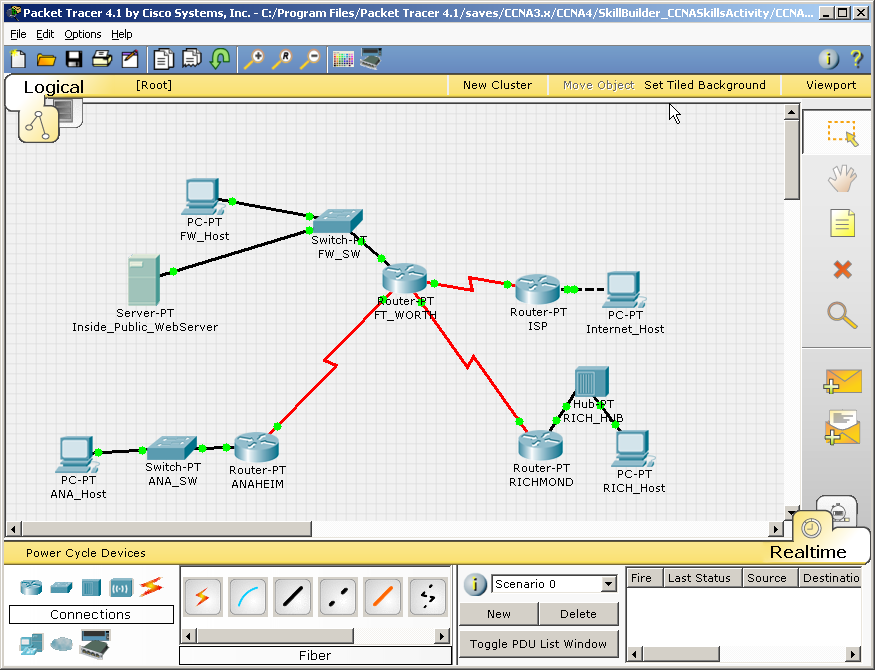
\includegraphics[width=12cm]{obrazky/packet-tracer}
\caption{Packet tracer}
\label{obr_packet-tracer}
\end{center}
\end{figure}



%------------------------------------------------------------------------------------------------------

\section{AdventNet Simulation Toolkit}

% AdventNet Simulation Toolkit 6
% AdventNet Simulation Toolkit 6 [7] je kompletný grafický softvérový simulátor
% zariadení a sietí s veľkou podporou viacerých protokolov, Cisco IOS zariadení a iných
% zariadení ako napr. rôzne Linux, či Windows 2000 servery. Tento simulátor je dostupný
% vo verzii nie len pre Windows, ale aj pre Linux a Solaris. Zo stránky sa dá po poskytnutí
% osobných údajov stiahnuť plne funkčná skúšobná verzia na 30 dní. Je síce limitovaná
% na maximálny počet 25 simulovaných prvkov, ale na začlenenie do tejto práce je postačujúca.

\uv{AdventNet Simulation Toolkit je kompletní grafický softwarový simulátor zařízení a sítí s velkou podporou mnohých protokolů, Cisco IOS zařízení a jiných zařízení jako např. různé Linux, či Windows 2000 servery.}\cite{resersni_bakalarka} Argumentem proti použití tohoto programu je především jeho cena, plná časově neomezená verze stojí od \$995 do \$14995 \footnote{k 23.5.2010}. K disposici je zkušební třicetidení verze.



%------------------------------------------------------------------------------------------------------

\section{Simulační software Omnet++}

\uv{Simulační systém OMNeT++ [11] je velmi propracovaný opensource nástroj pro simulaci prakticky čehokoliv. OMNeT++ je postaven na modulární architektuře, takže při správných knihovnách (modulech) může simulovat počítačovou síť. Systém dokáže simulovat Cisco IOS i počítač postavený na linuxu.}\cite{resersni_bakalarka}. Systém se však hodí spíše pro simulaci zatížení sítě a pro simulaci síťových protokolů. K výukovým účelům není příliš vhodný kvůli své složitosti.

Více se tímto simulátorem zabýval Bc. Jan Michek v~rámci své diplomové práce Emulátor počítačové sítě \cite{reserse:omnet_dp}.

% omnet
\begin{figure}[h]
\begin{center}
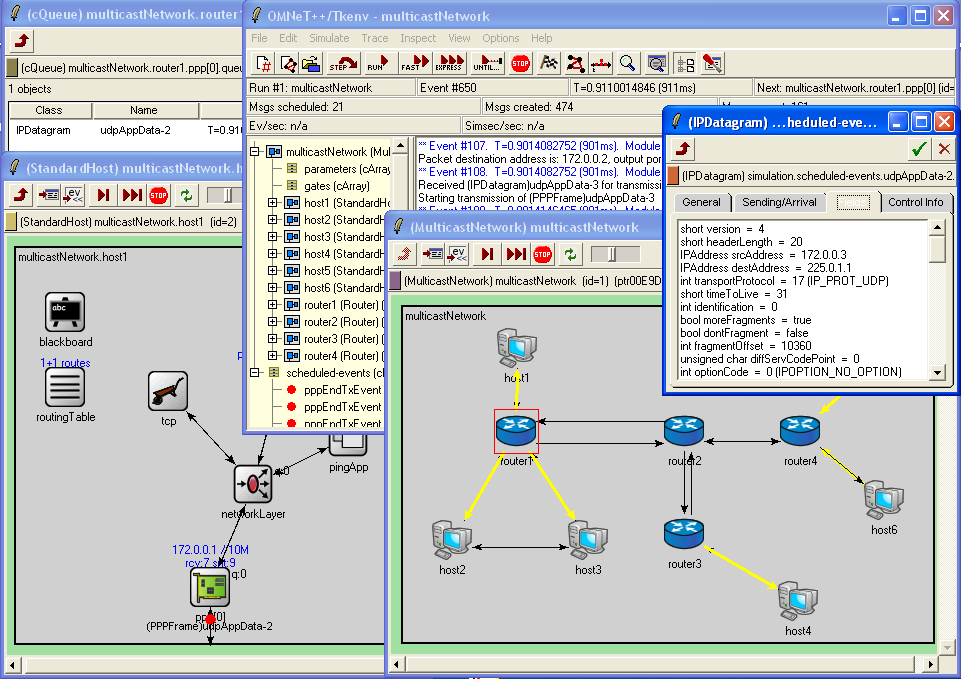
\includegraphics[width=12cm]{obrazky/omnet}
\caption{Omnet++}
\label{obr_omnet}
\end{center}
\end{figure}



%------------------------------------------------------------------------------------------------------

\section{Závěr}

Tvůrci simulačních programů dávají většinou přednost simulaci sítí založených na síťových prvcích ood firmy Cisco. Podporují-li i počítače s linuxem, ani o tom moc nepíší. Většina simulátorů je studentům nedostupná kvůli své ceně. Studenti předmětu PSI budou simulátor potřebovat pravděpodobně jen několikrát za semestr a je nesmyslné, aby si škola, nebo sami studenti kupovali kvůli několika použitím licenci.

